\section{Моделирование нагрева резиста при экспонировании} \label{sec:sim_heating}

Выделение энергии в резисте при экспонировании может приводить к повышению его температуры, что может повлиять на масштаб процессов деполимеризации, диффузии и растекания. В работах по моделированию нагрева резиста при экспонировании часто рассматривается случай плоского слоя резиста, расположенного на поверхности полубесконечной подложки~\cite{Cui_heating} (рисунок~\ref{fig:heating_paper}). В этом случае уравнение теплопроводности принимает следующий вид:
\begin{equation} \label{eq:heat_diffusion}
	\begin{aligned}
		& \frac{\partial T_1}{\partial t}-k_1\left(\frac{\partial^2 T_1}{\partial x^2}+\frac{\partial^2 T_1}{\partial y^2}+\frac{\partial^2 T_1}{\partial z^2}\right) = h(x, y, z, t), \quad 0 < z \leqslant d, \\
		& \frac{\partial T_2}{\partial t}-k_2\left(\frac{\partial^2 T_2}{\partial x^2}+\frac{\partial^2 T_2}{\partial y^2}+\frac{\partial^2 T_2}{\partial z^2}\right) = h(x, y, z, t), \quad d \leqslant z < \infty.
	\end{aligned}
\end{equation}
Здесь $d$ -- толщина слоя резиста, $k_i = D_i / \rho_i c_{\mathrm{v} i}$ ($i=1,2$), $h=S / \rho c_\mathrm{v}$, $D_i$, $\rho_i$ и $c_{\mathrm{v} i}$  -- коэффициент теплопроводности, плотность и удельная теплоемкость резиста ($i=1$) или подложки ($i=2$). Величина $S$, определяющая скорость выделения тепла в резисте при экспонировании, может быть рассчитана по формуле
\begin{equation}
	S(x, y, z, t)=\frac{E_0 Q \lambda(\xi)}{R_{\mathrm{g}} t_{\mathrm{e}}},
\end{equation}
где $E_0$ -- энергия электронного пучка, $Q$, $t_\mathrm{e}$ -- доза и время экспонирования, соответственно, $R_\mathrm{g}$ -- радиус Грюна:
\begin{equation}
	R_{\mathrm{g}}=\frac{4.6 \times 10^{-2}}{\rho} E_0^{1.75},
\end{equation}
а для определения энергии, выделившейся в резисте на глубине $z$ используется эмпирическая функция $\lambda(\xi)$ с параметрами $b_i$~\cite{Everhart_lambda}:
\begin{equation}
	\begin{aligned}
	& \lambda(\xi) = b_0+b_1 \xi+b_2 \xi^2+b_3 \xi^3, \\
	& \xi=z/R_\mathrm{g}.
	\end{aligned}
\end{equation}

\begin{figure}
	\centering
	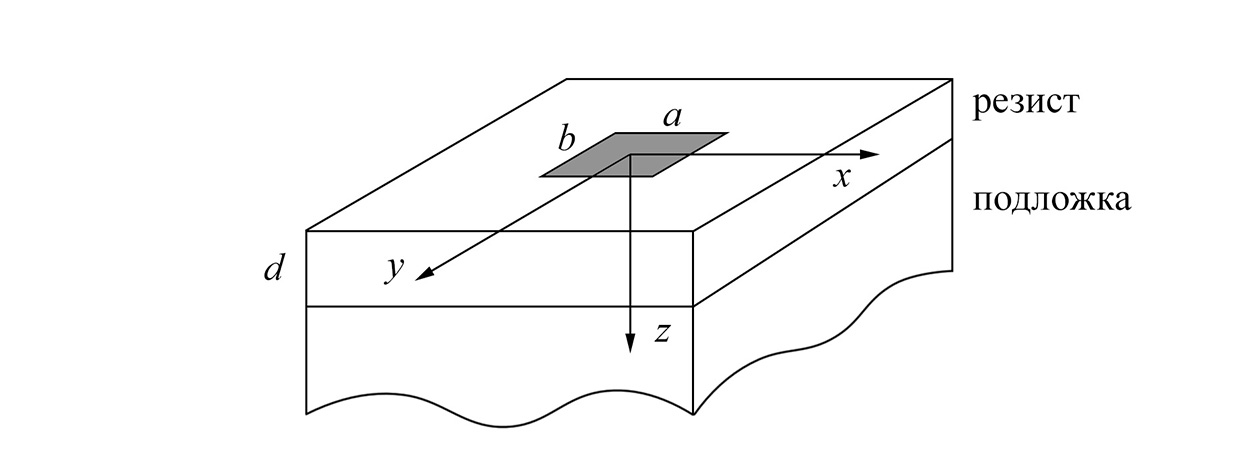
\includegraphics[width=0.9\linewidth]{jpg/heating_paper_200}
	\caption{Система координат и обозначения, используемые при моделировании нагрева резиста в процессе экспонировании~\cite{Cui_heating}.}
	\label{fig:heating_paper}
\end{figure}
Граничные условия для уравнения~\ref{eq:heat_diffusion} имеют вид:
\begin{equation} \label{eq:heat_diff_eq_conditions}
	\begin{aligned}
		\left.\frac{\partial T_1}{\partial z}\right|_{z=0} &= 0, \\
		D_1 \left.\frac{\partial T_1}{\partial z}\right|_{z=d} &= D_2 \left.\frac{\partial T_2}{\partial z}\right|_{z=d}, \\
		\left.T_1\right|_{z=d} &= \left.T_2\right|_{z=d}, \\
		\lim _{z \rightarrow \infty} T_2 &= 0, \\
		\lim _{(x,y) \rightarrow (\infty, \infty)} T_1 &= \lim _{(x,y), \rightarrow (\infty, \infty)} T_2 = 0.
	\end{aligned}
\end{equation}
Решение уравнения~\ref{eq:heat_diffusion} с граничными условиями~\ref{eq:heat_diff_eq_conditions} выражается в следующем виде:
\begin{equation} \label{eq:heat_final_equation}
	\begin{split}
		T(x, y, z, t) = & \int_0^{t_\mathrm{e}} \mathrm{d} t^{\prime} \int_{-a / 2}^{a / 2} d x^{\prime} \int_{-b / 2}^{b / 2} d y^{\prime} \int_0^d h\left(x^{\prime}, y^{\prime}, z^{\prime}, t^{\prime}\right) \times \\ & \times G\left(x, x^{\prime}, y, y^{\prime}, z, z^{\prime}, t, t^{\prime}\right) d z^{\prime},
	\end{split}
\end{equation}
\begin{equation}
	G=\frac{1}{4 \pi k\left(t-t^{\prime}\right)} \exp \left(-\frac{\left(x-x^{\prime}\right)^2+\left(y-y^{\prime}\right)^2}{4 k\left(t-t^{\prime}\right)}\right) g,
\end{equation}
где для слоя резиста функция $g$ задается выражением
\begin{equation}
	\begin{aligned}
		&g_1=\frac{1}{2 \sqrt{\pi k_1\left(t-t^{\prime}\right)}}\left[\exp \left(-\frac{\left(z-z^{\prime}\right)^2}{4 k_1\left(t-t^{\prime}\right)}\right)\right.+\exp \left(-\frac{\left(z+z^{\prime}\right)^2}{4 k_1\left(t-t^{\prime}\right)}\right)+\\
		&+\frac{2 \sigma K}{1+\sigma} \exp \left(-\frac{\left[d+z+K\left(d-z^{\prime}\right)\right]^2}{4 k_1\left(t-t^{\prime}\right)}\right)+\frac{2 \sigma K}{1+\sigma} \exp \left(-\frac{\left[d-z+K\left(d-z^{\prime}\right)\right]^2}{4 k_1\left(t-t^{\prime}\right)}\right)+\\
		&+\frac{2 \sigma K}{1+\sigma} \sum_{n=1}^{\infty}(-\alpha)^n \exp \left(-\frac{\left[(2 n+1) d+z+K\left(d-z^{\prime}\right)\right]^2}{4 k_1\left(t-t^{\prime}\right)}\right)+\\
		&+\frac{2 \sigma K}{1+\sigma} \sum_{n=1}^{\infty}(-\alpha)^n \exp \left(-\frac{\left[(2 n+1) d-z+K\left(d-z^{\prime}\right)\right]^2}{4 k_1\left(t-t^{\prime}\right)}\right)+\\
		&+\sum_{n=1}^{\infty}(-\alpha)^n \exp \left(-\frac{\left(z+z^{\prime}+2 n d\right)^2}{4 k_1\left(t-t^{\prime}\right)}\right)+\sum_{n=1}^{\infty}(-1)^n \alpha^{n-1} \exp \left(-\frac{\left(z-z^{\prime}+2 n d\right)^2}{4 k_1\left(t-t^{\prime}\right)}\right)+\\
		&+\sum_{n=1}^{\infty}(-1)^n \alpha^{n-1} \exp \left(-\frac{\left(2 n d-z^{\prime}-z\right)^2}{4 k_1\left(t-t^{\prime}\right)}\right)+\left.\sum_{n=1}^{\infty}(-\alpha)^n \exp \left(-\frac{\left(2 n d+z^{\prime}-z\right)^2}{4 k_1\left(t-t^{\prime}\right)}\right)\right]
	\end{aligned}
\end{equation}
и для подложки -- выражением
\begin{equation}
	\begin{aligned}
		g_2=& \frac{1}{2 \sqrt{\pi k_2\left(t-t^{\prime}\right)}}\left[(2-\eta) \exp \left(-\frac{\left(z-z^{\prime}\right)^2}{4 k_2\left(t-t^{\prime}\right)}\right)\right.-\\
		&-\eta\left(1+\frac{1}{\alpha}\right) \sum_{n=1}^{\infty}(-\alpha)^n \exp \left(-\frac{\left(2 n K^{\prime} d+z^{\prime}-z\right)^2}{4 k_2\left(t-t^{\prime}\right)}\right)+\\
		&+\beta \sum_{n=1}^{\infty}(-\alpha)^{n-1} \exp \left(-\frac{\left\{(z-d)-K^{\prime}\left[z^{\prime}+(2 n-1) d\right]\right\}^2}{4 k_2\left(t-t^{\prime}\right)}\right)-\\
		&-\beta \sum_{n=1}^{\infty}(-\alpha)^{n-1}\left.\exp \left(-\frac{\left\{(z-d)-K^{\prime}\left[z^{\prime}-(2 n+1) d\right]\right\}^2}{4 k_2\left(t-t^{\prime}\right)}\right)\right],
	\end{aligned}
\end{equation}
где
\begin{equation}
	\begin{aligned}
		&K=\sqrt{\frac{k_1}{k_2}}, \quad K^{\prime}=\frac{1}{K}, \quad \sigma=\frac{D_2}{D_1} \sqrt{\frac{k_1}{k_2}}, \alpha=\frac{\sigma+1}{\sigma-1},\\
		&\eta=\frac{2 \sigma K \theta}{1+\sigma}, \quad \beta=\frac{1+\alpha}{\sigma} \theta=\frac{D_1}{D_2} \frac{k_2}{k_1}.
	\end{aligned}
\end{equation}
